\begin{figure}
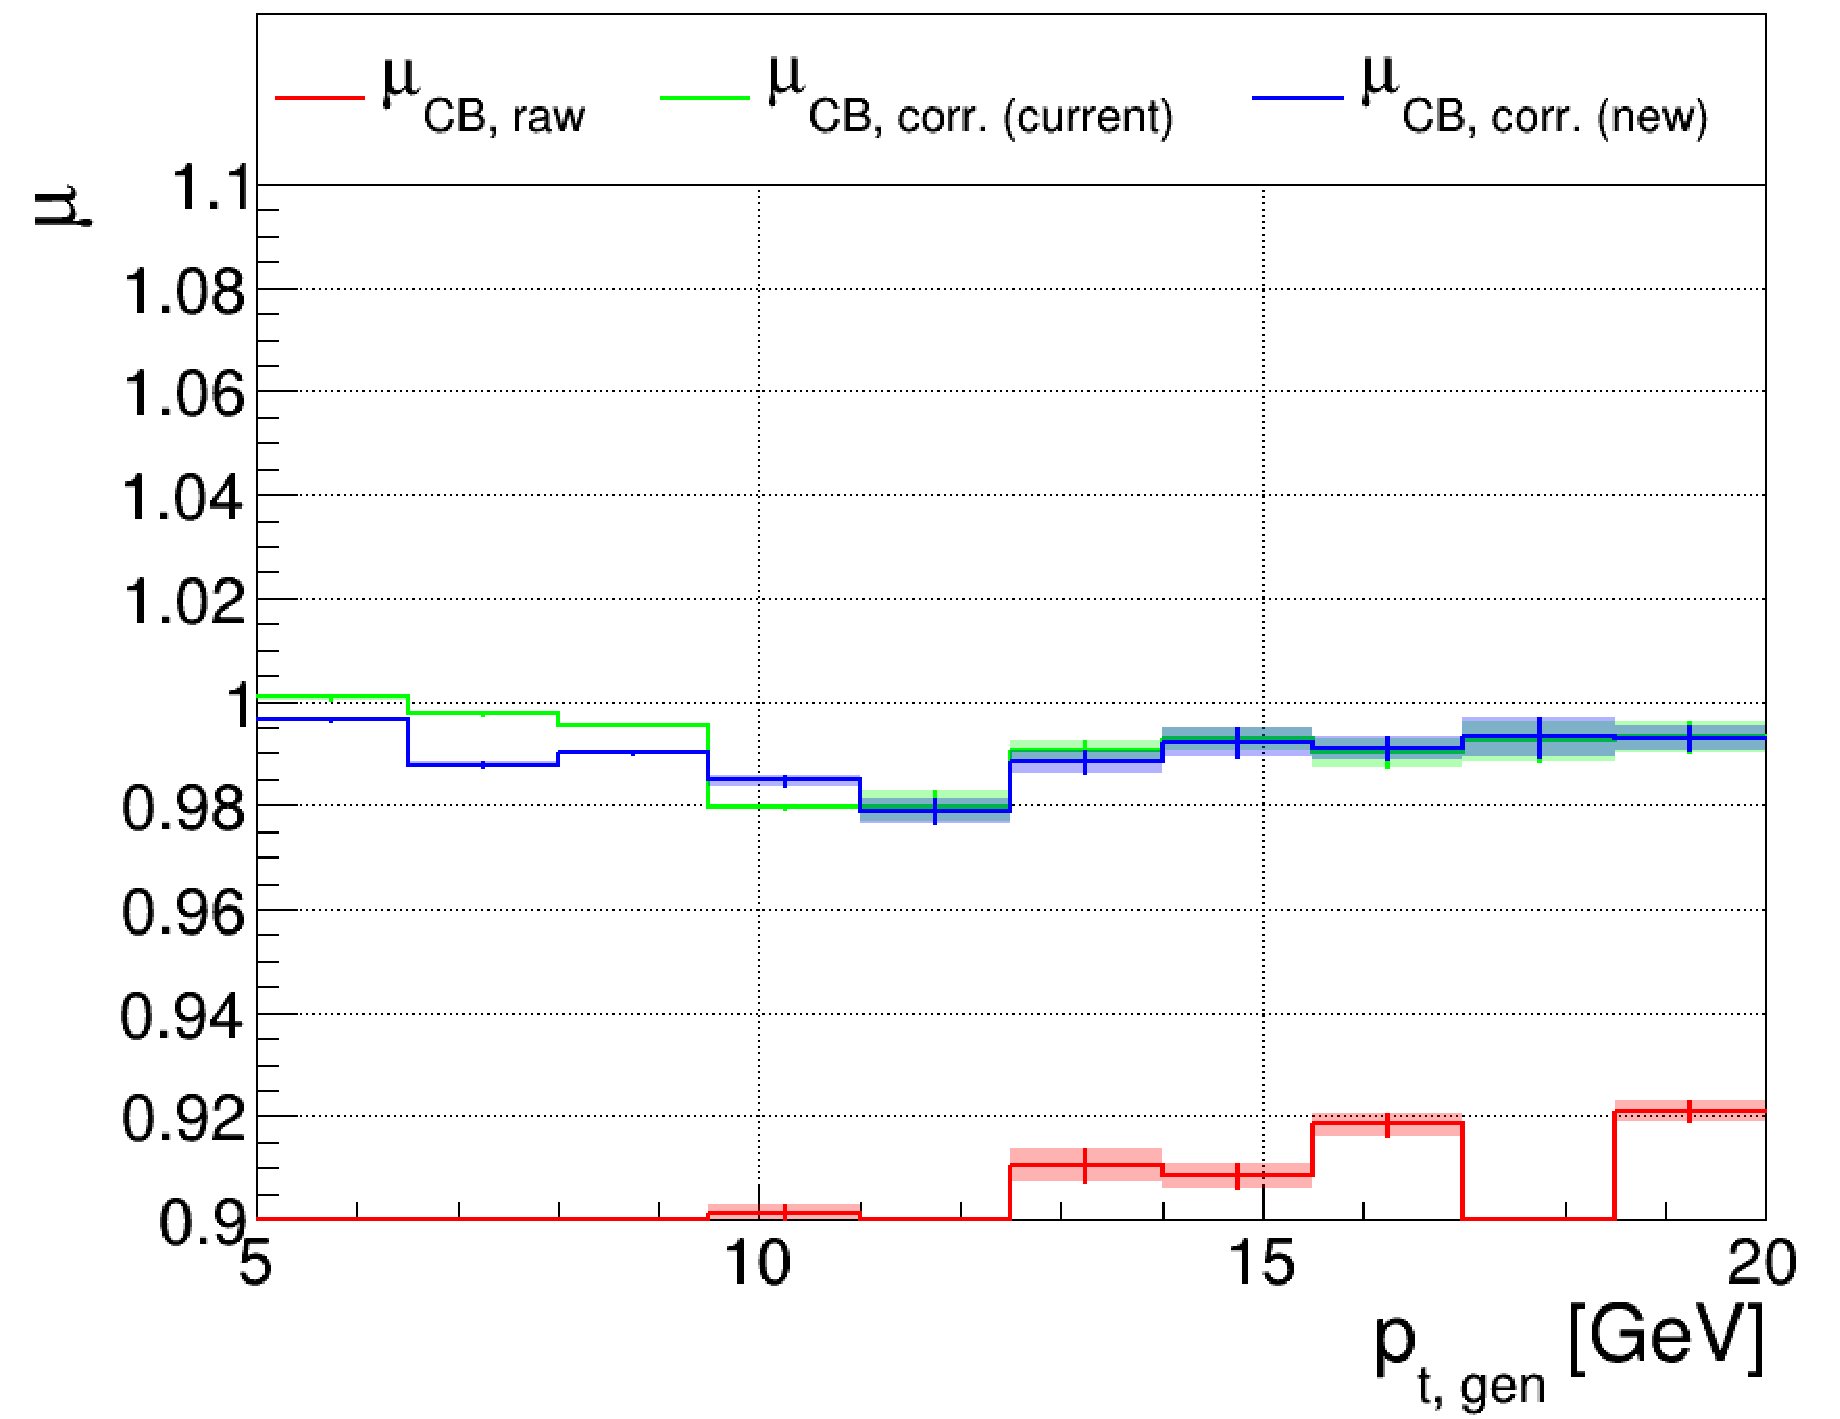
\includegraphics[width=0.495\textwidth]{./plots_pdf/ECAL_plots/plotsPU/EE/FULL/pdf/GENPT/EEFULL_GENPT_0005_0020_MuOverBins.pdf}
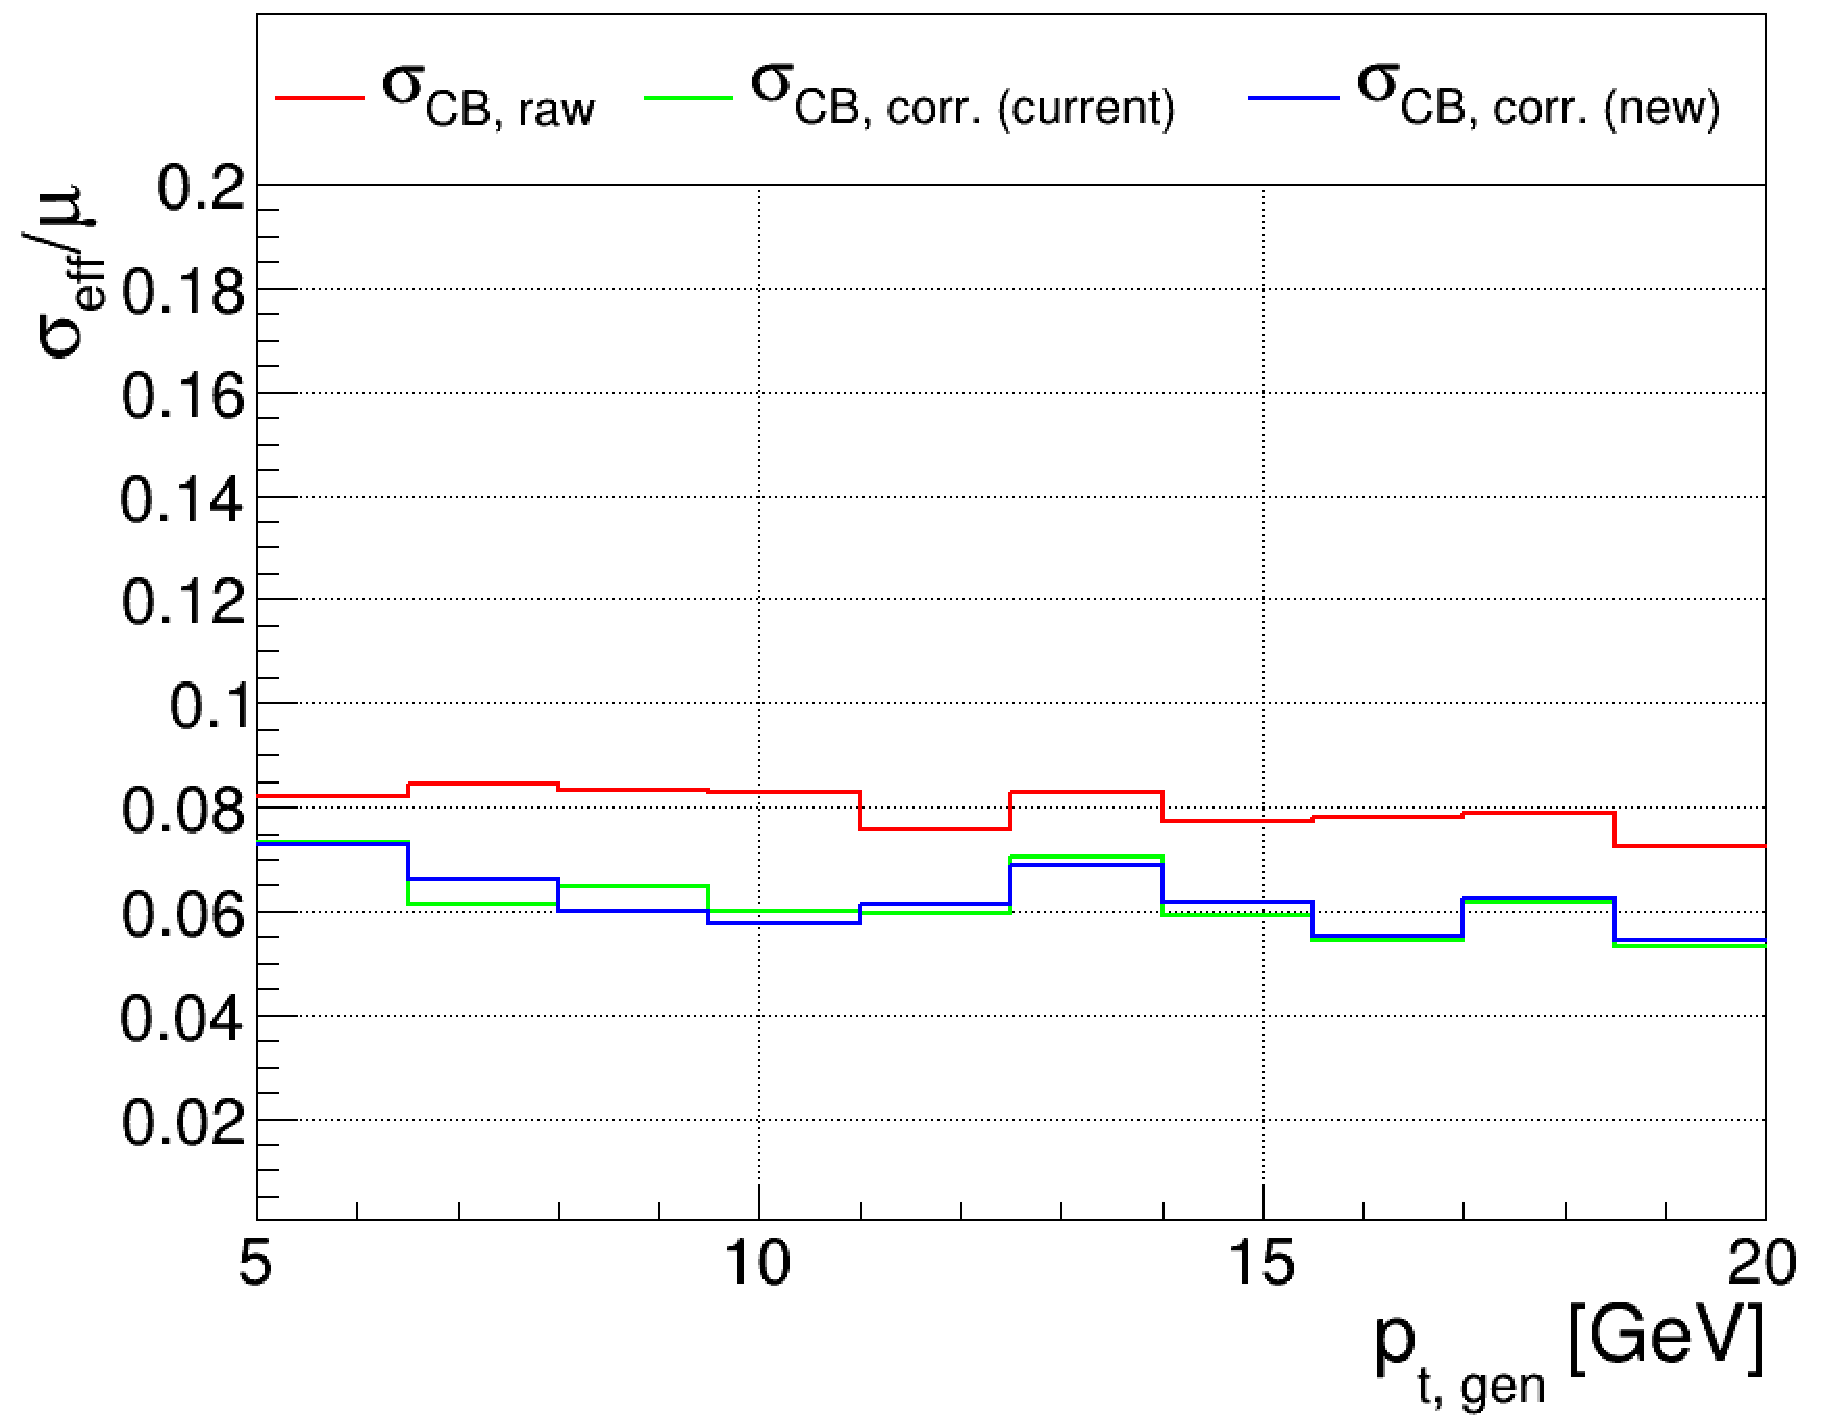
\includegraphics[width=0.495\textwidth]{./plots_pdf/ECAL_plots/plotsPU/EE/FULL/pdf/GENPT/EEFULL_GENPT_0005_0020_EffSigmaOverBins.pdf}
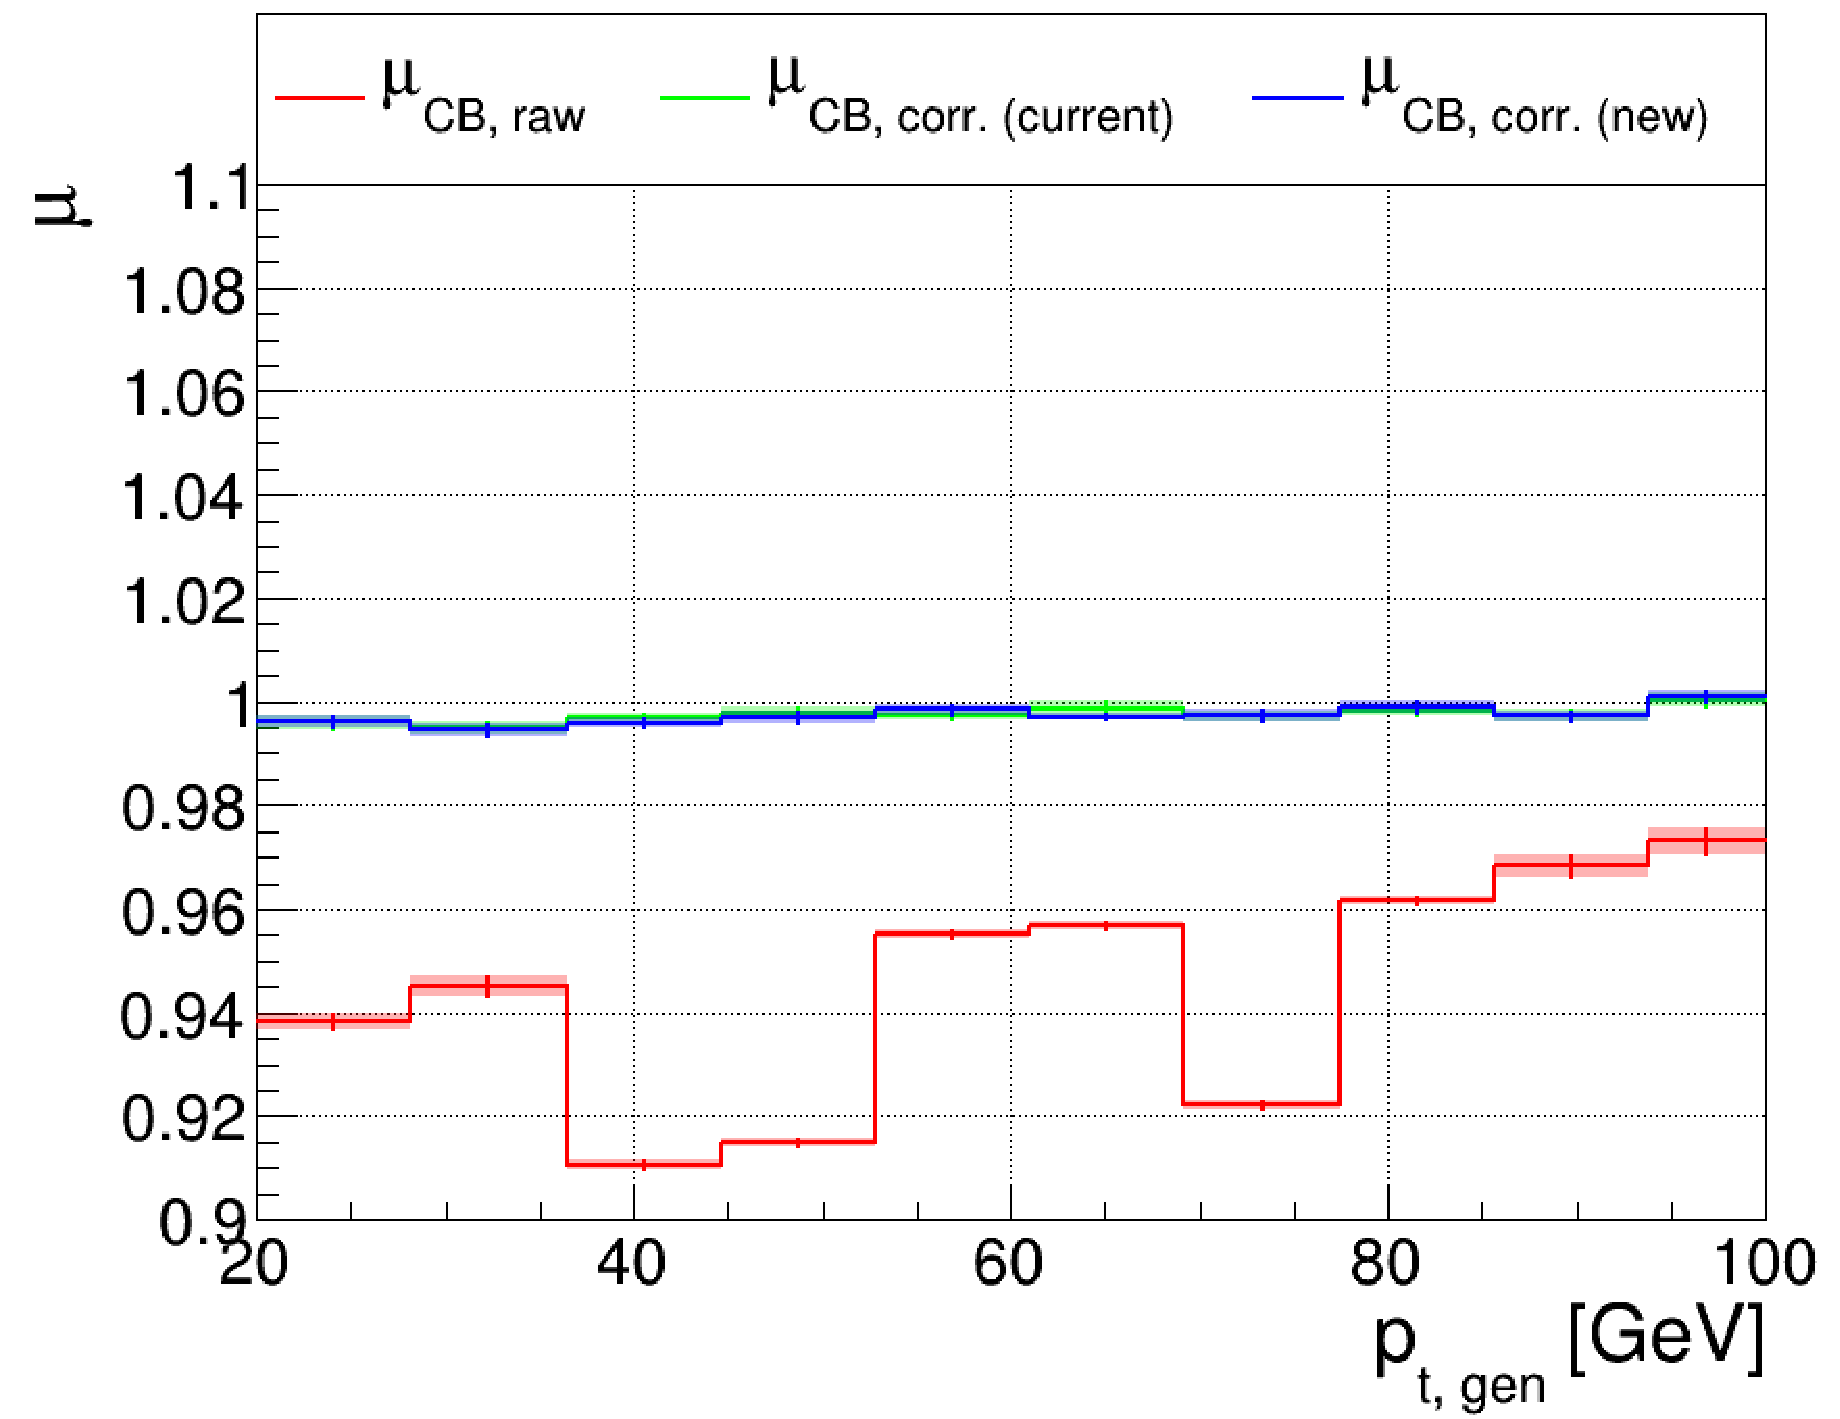
\includegraphics[width=0.495\textwidth]{./plots_pdf/ECAL_plots/plotsPU/EE/FULL/pdf/GENPT/EEFULL_GENPT_0020_0100_MuOverBins.pdf}
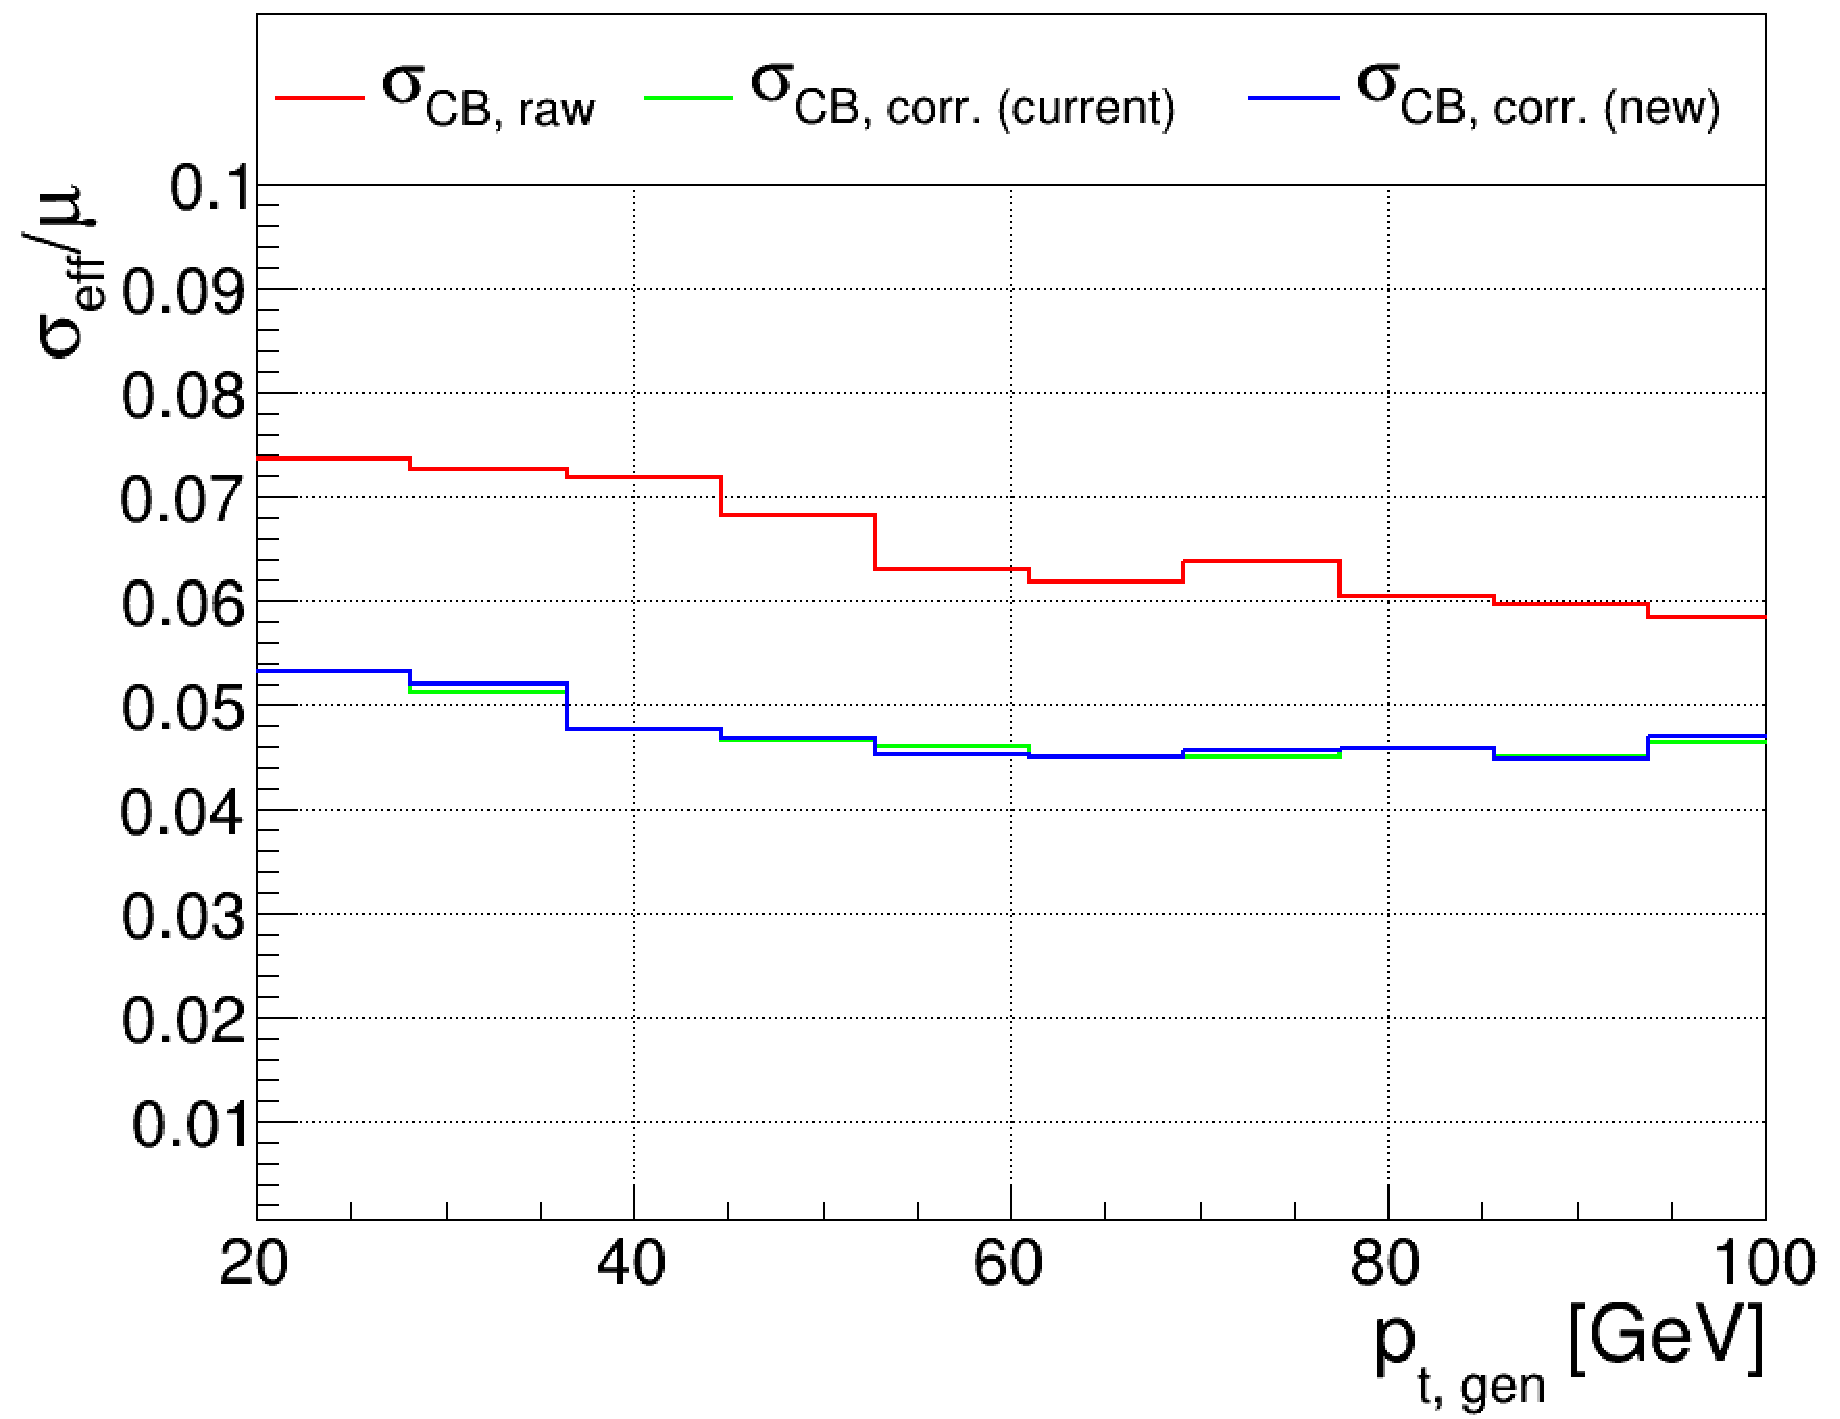
\includegraphics[width=0.495\textwidth]{./plots_pdf/ECAL_plots/plotsPU/EE/FULL/pdf/GENPT/EEFULL_GENPT_0020_0100_EffSigmaOverBins.pdf}
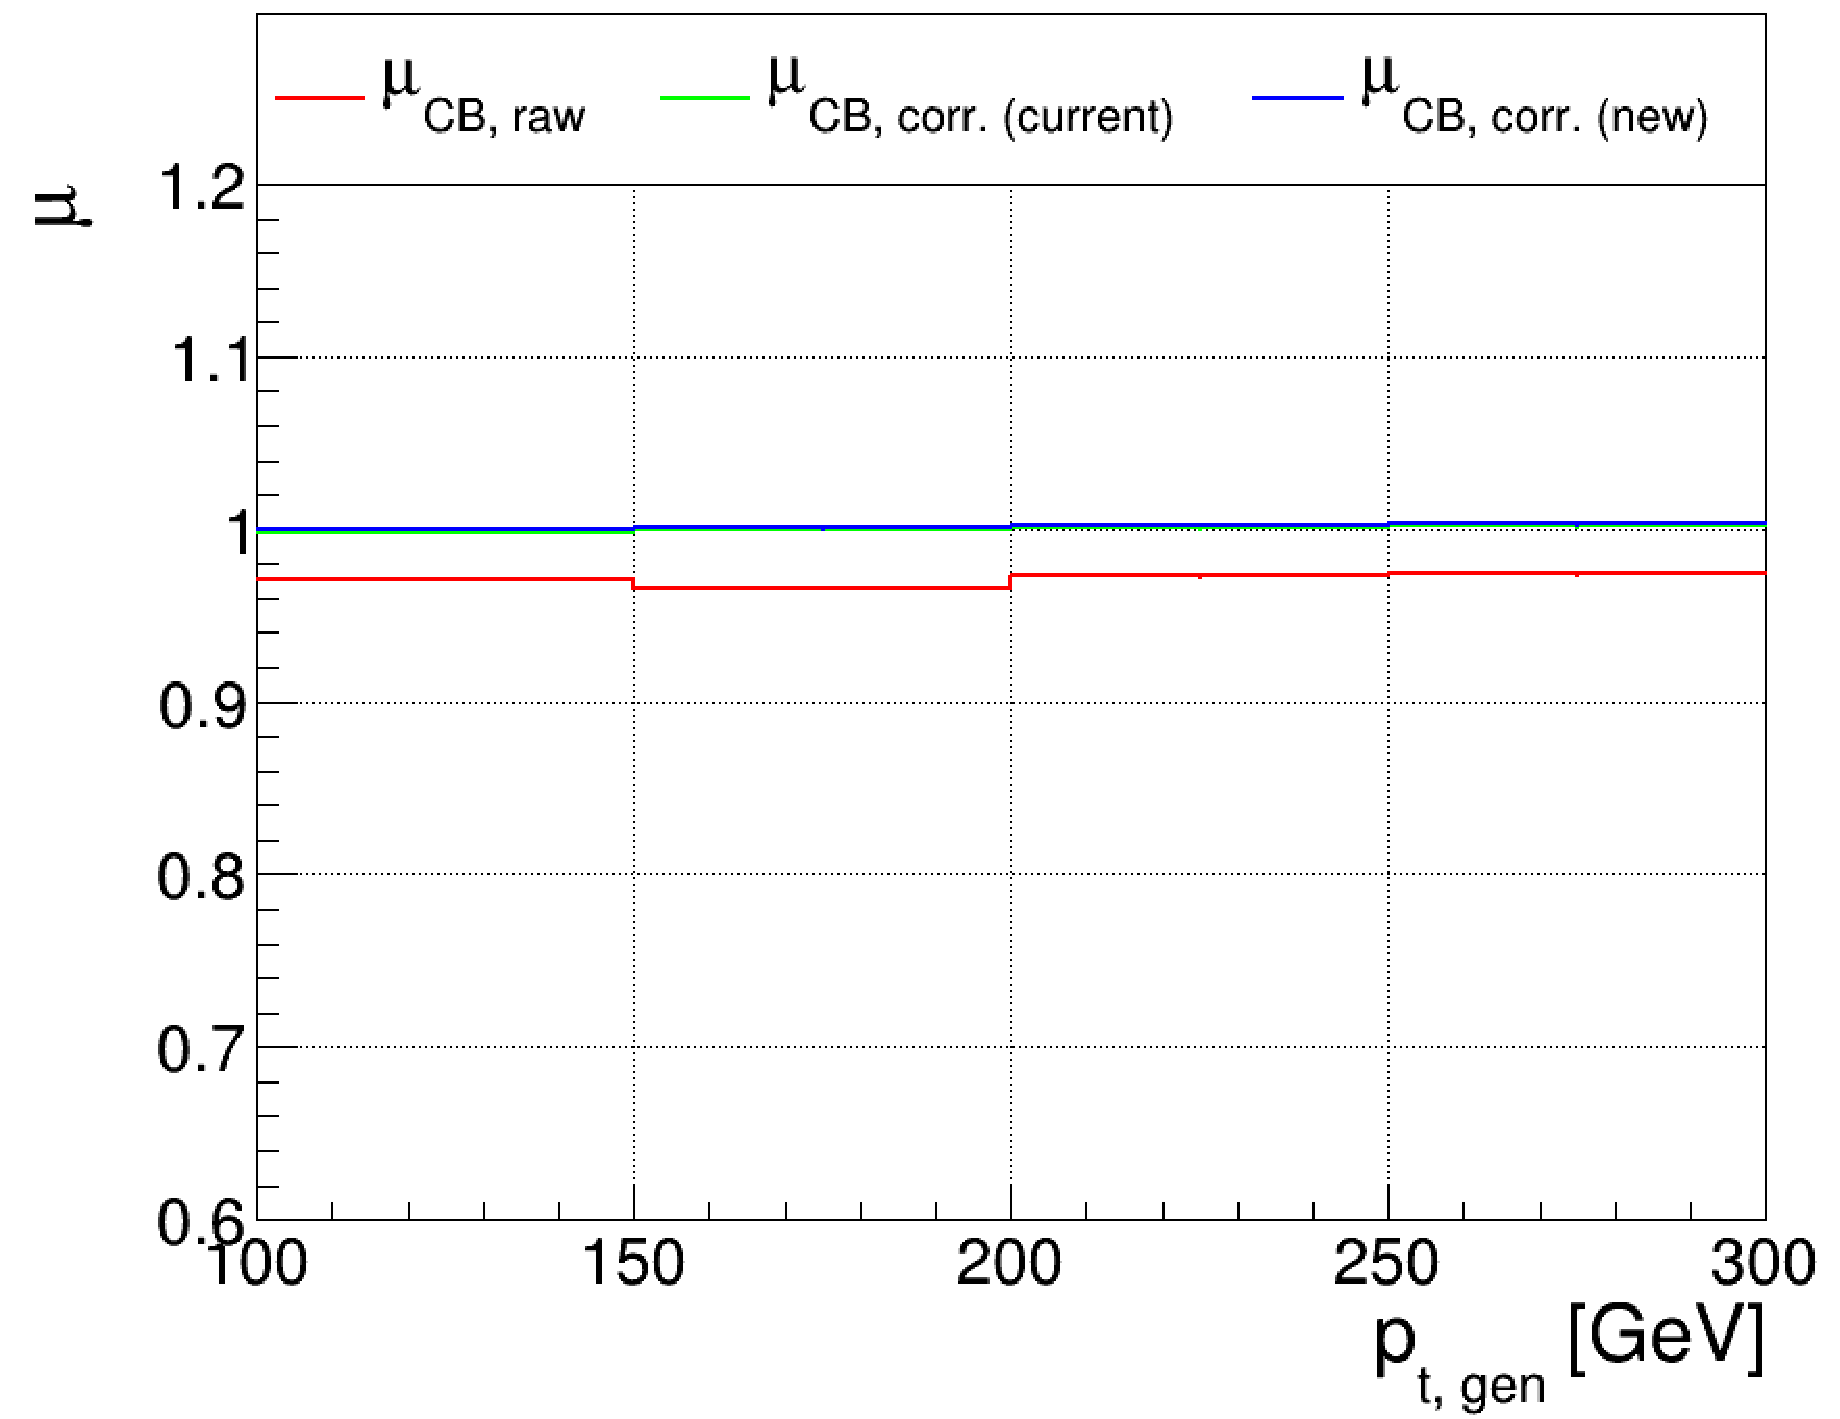
\includegraphics[width=0.495\textwidth]{./plots_pdf/ECAL_plots/plotsPU/EE/FULL/pdf/GENPT/EEFULL_GENPT_0100_0300_MuOverBins.pdf}
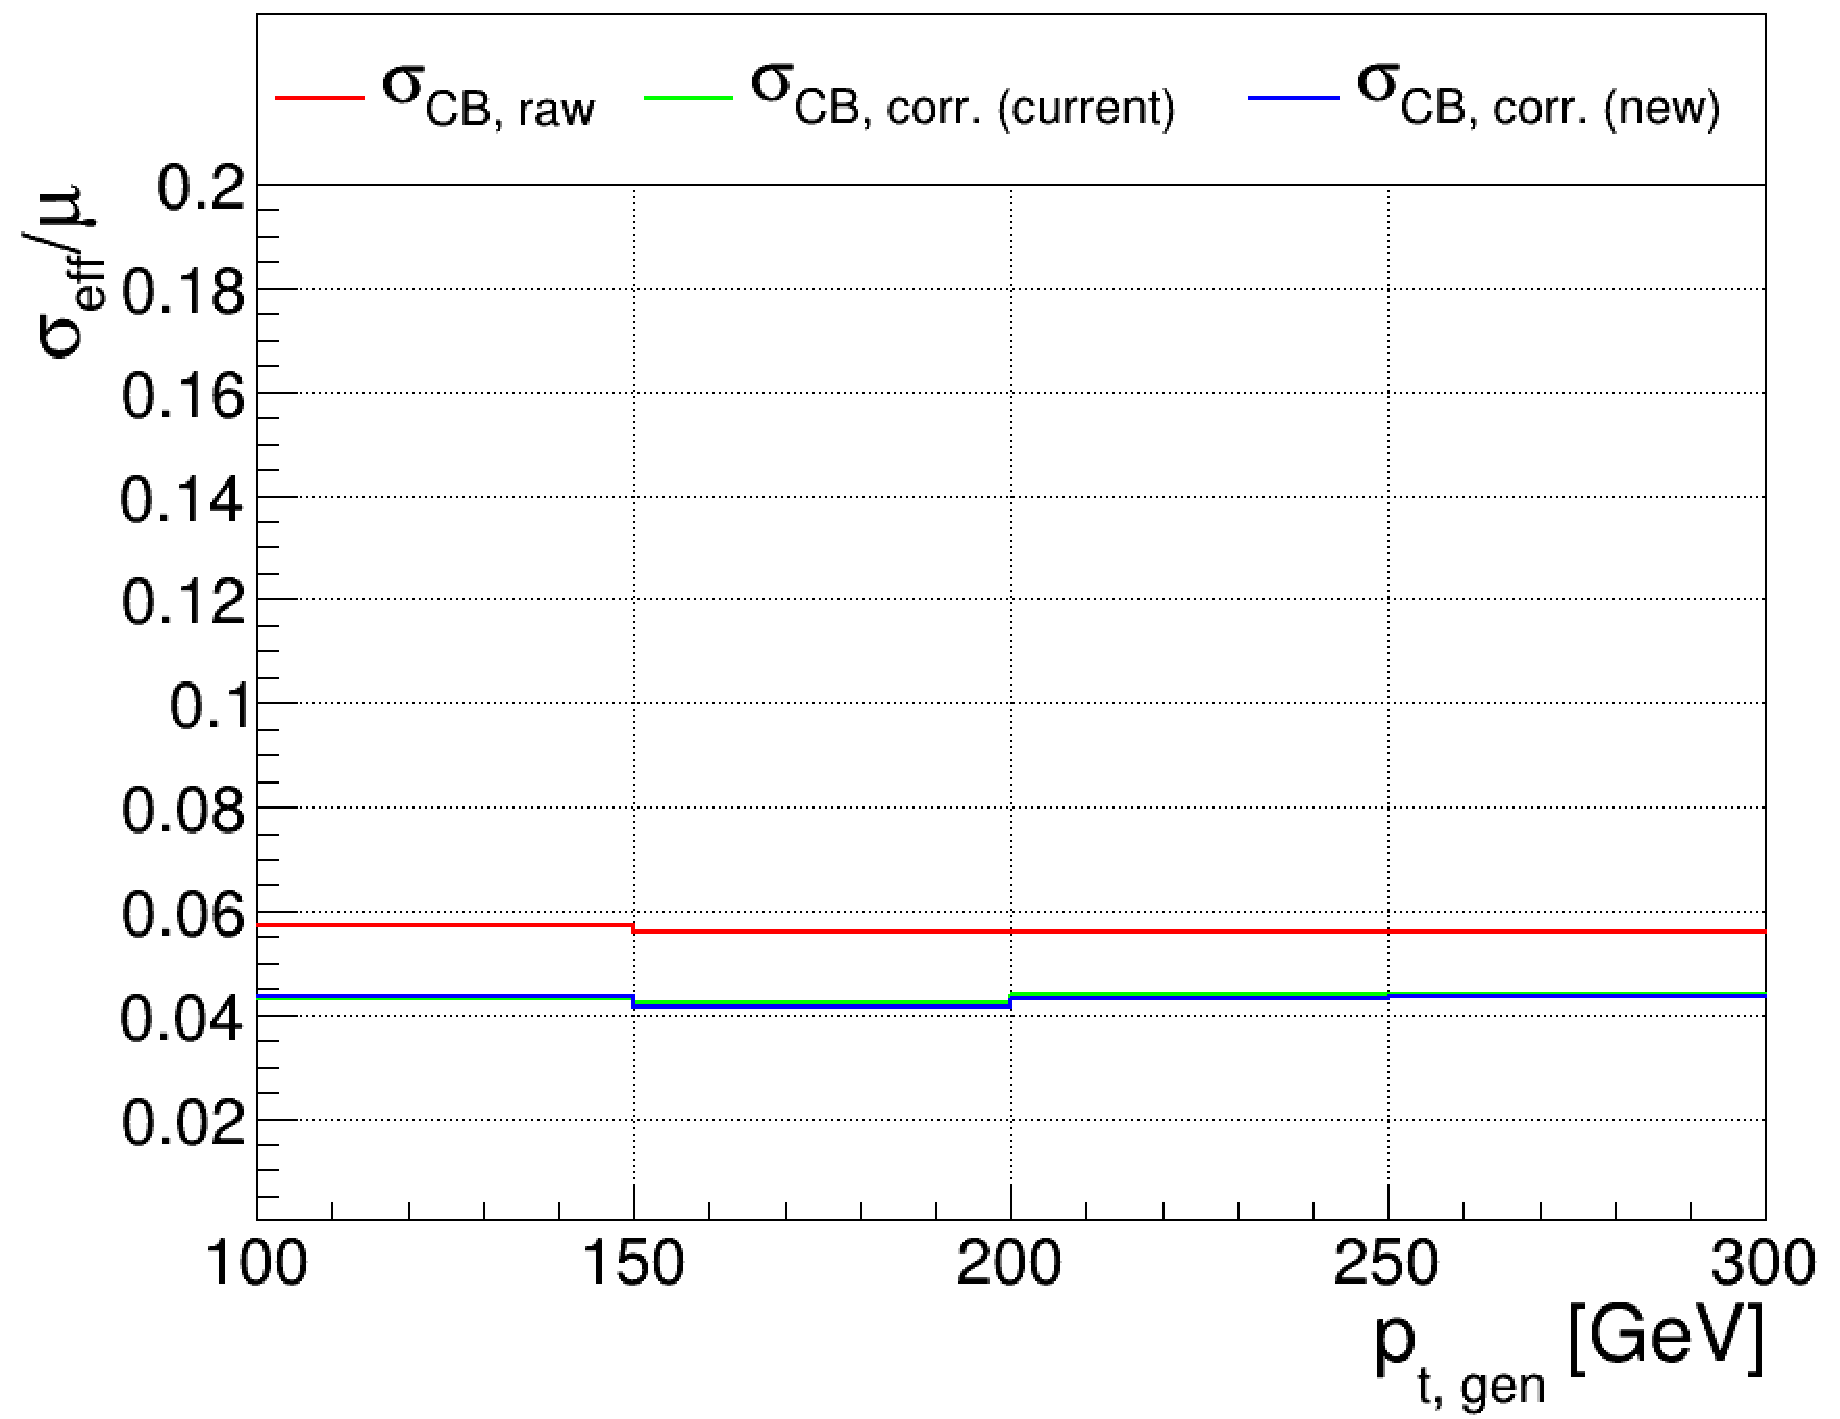
\includegraphics[width=0.495\textwidth]{./plots_pdf/ECAL_plots/plotsPU/EE/FULL/pdf/GENPT/EEFULL_GENPT_0100_0300_EffSigmaOverBins.pdf}

\caption [$\mu$ ($\sigma_\mathrm{eff}$) vs. \pt of PF ECAL cluster - EE full readout PU scenario]{Mean response (resolution) defined by raw PF ECAL clusters (red), the calibration derived earlier in Run~3 based on 126X (green), and the new correction from the 2024 simulation sample based on 133X (blue). (top) low \pt, (middle) mid \pt, (bottom) high \pt in EE region full readout PU scenario.}
\label{fig:PU_EEFULL_pt}
\end{figure}


\begin{figure}
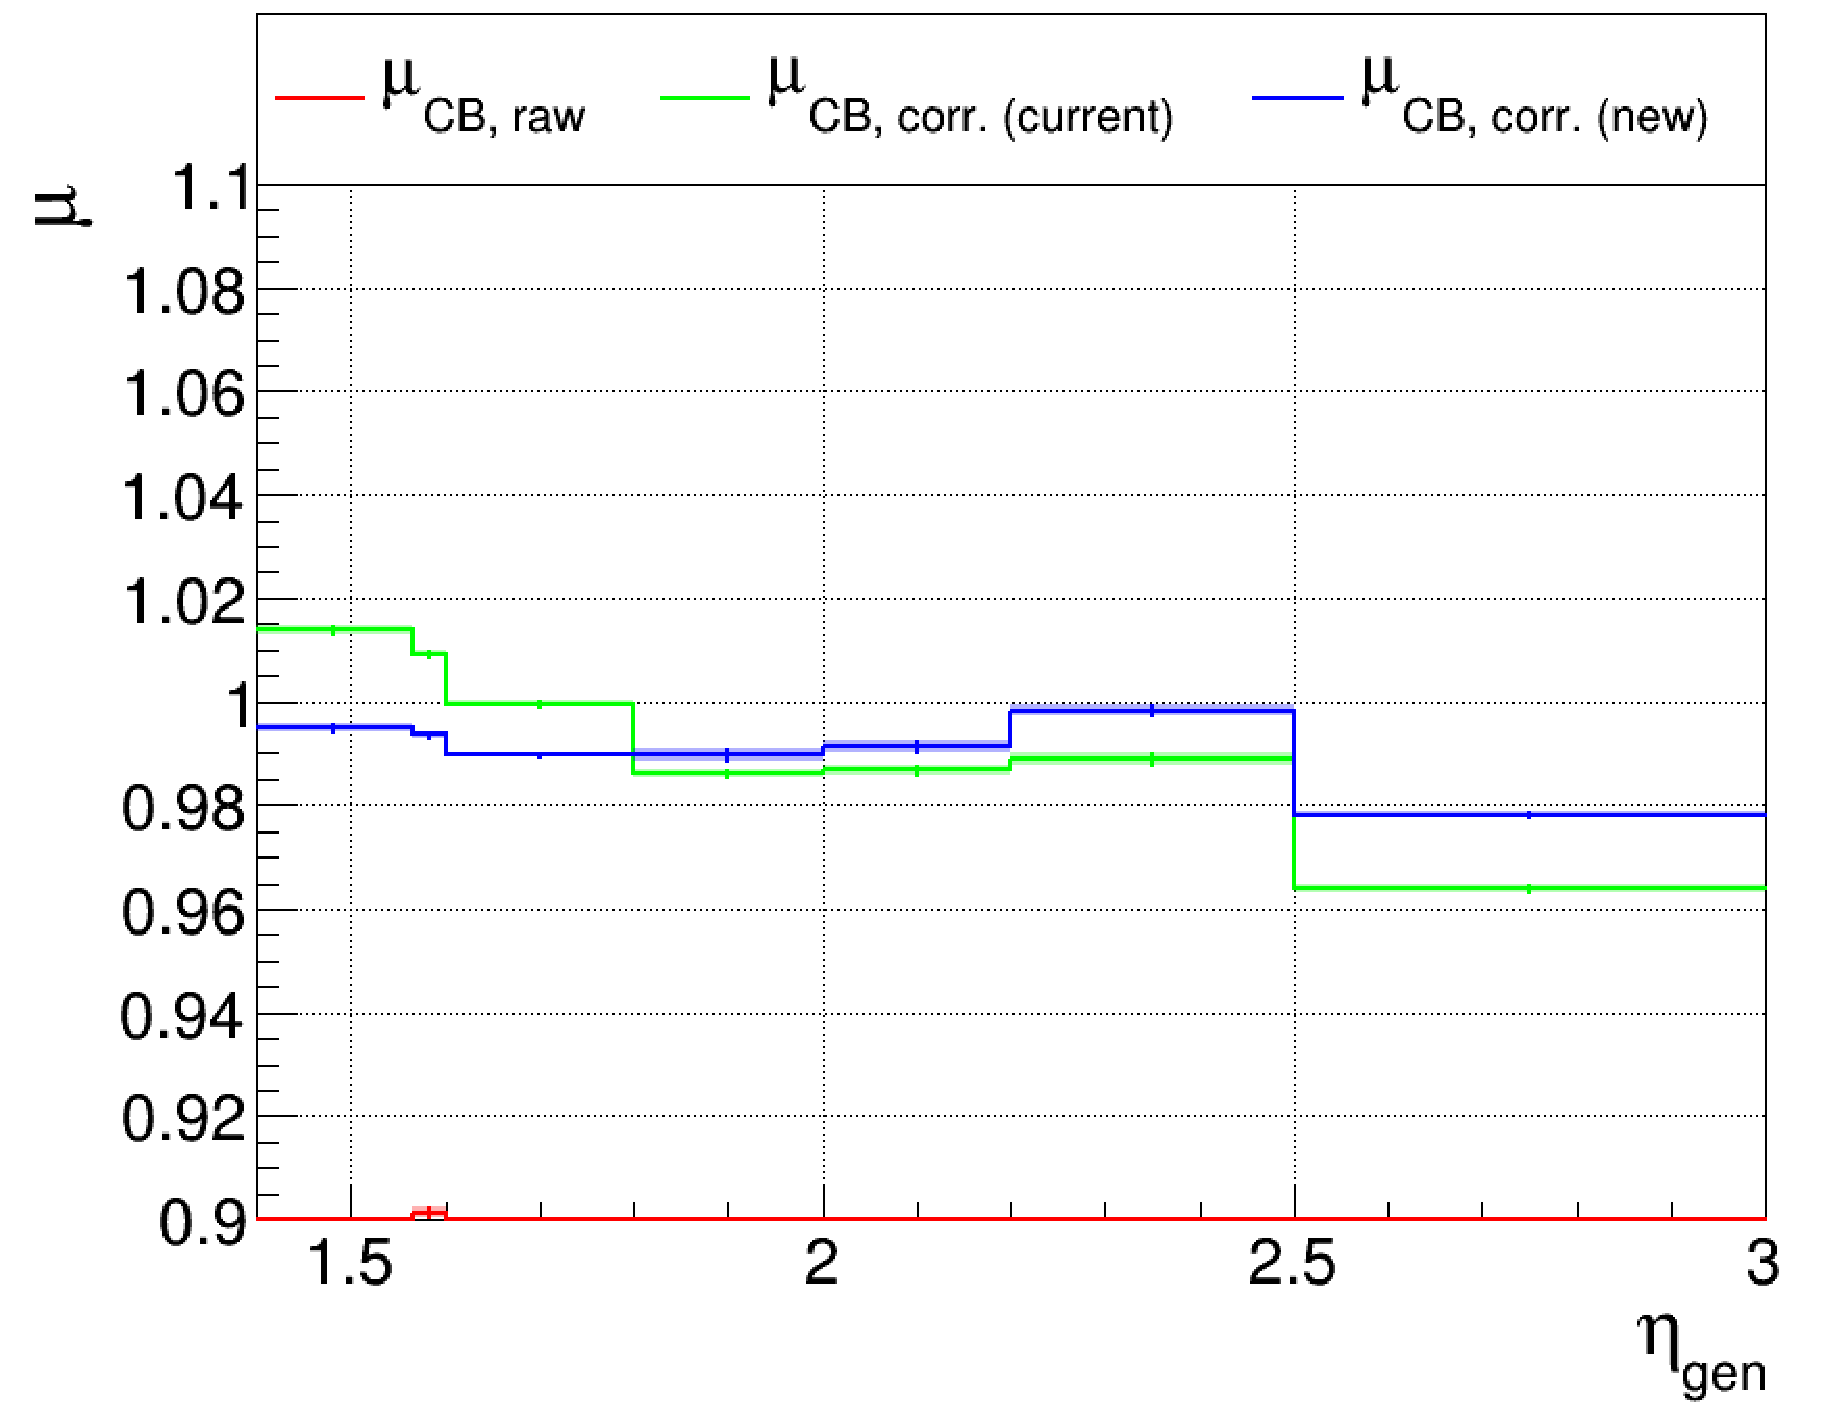
\includegraphics[width=0.495\textwidth]{./plots_pdf/ECAL_plots/plotsPU/EE/FULL/pdf/GENETA/EEFULL_GENETA_0005_0020_MuOverBins.pdf}
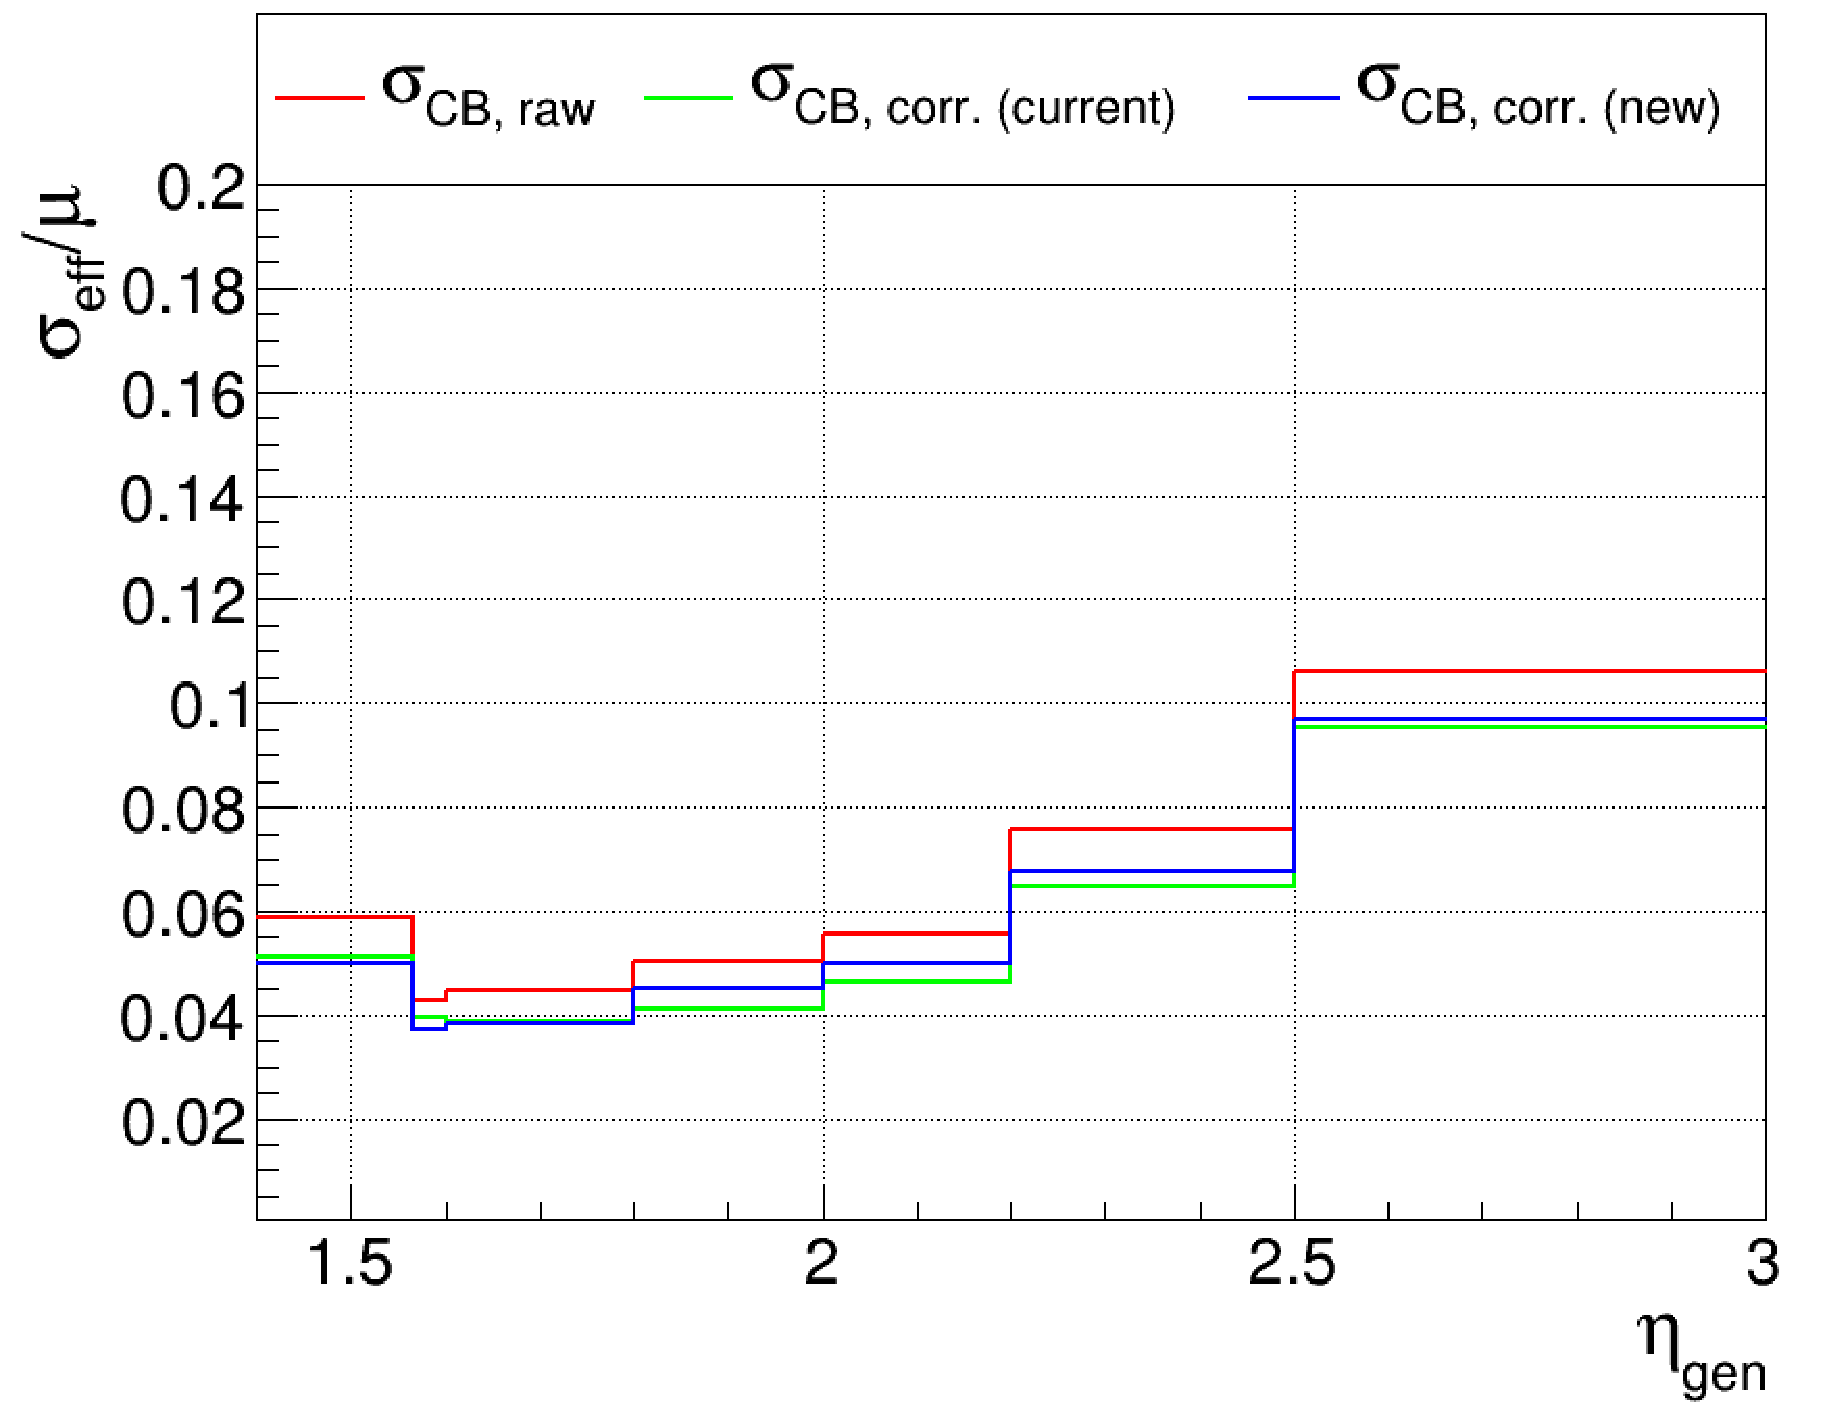
\includegraphics[width=0.495\textwidth]{./plots_pdf/ECAL_plots/plotsPU/EE/FULL/pdf/GENETA/EEFULL_GENETA_0005_0020_EffSigmaOverBins.pdf}
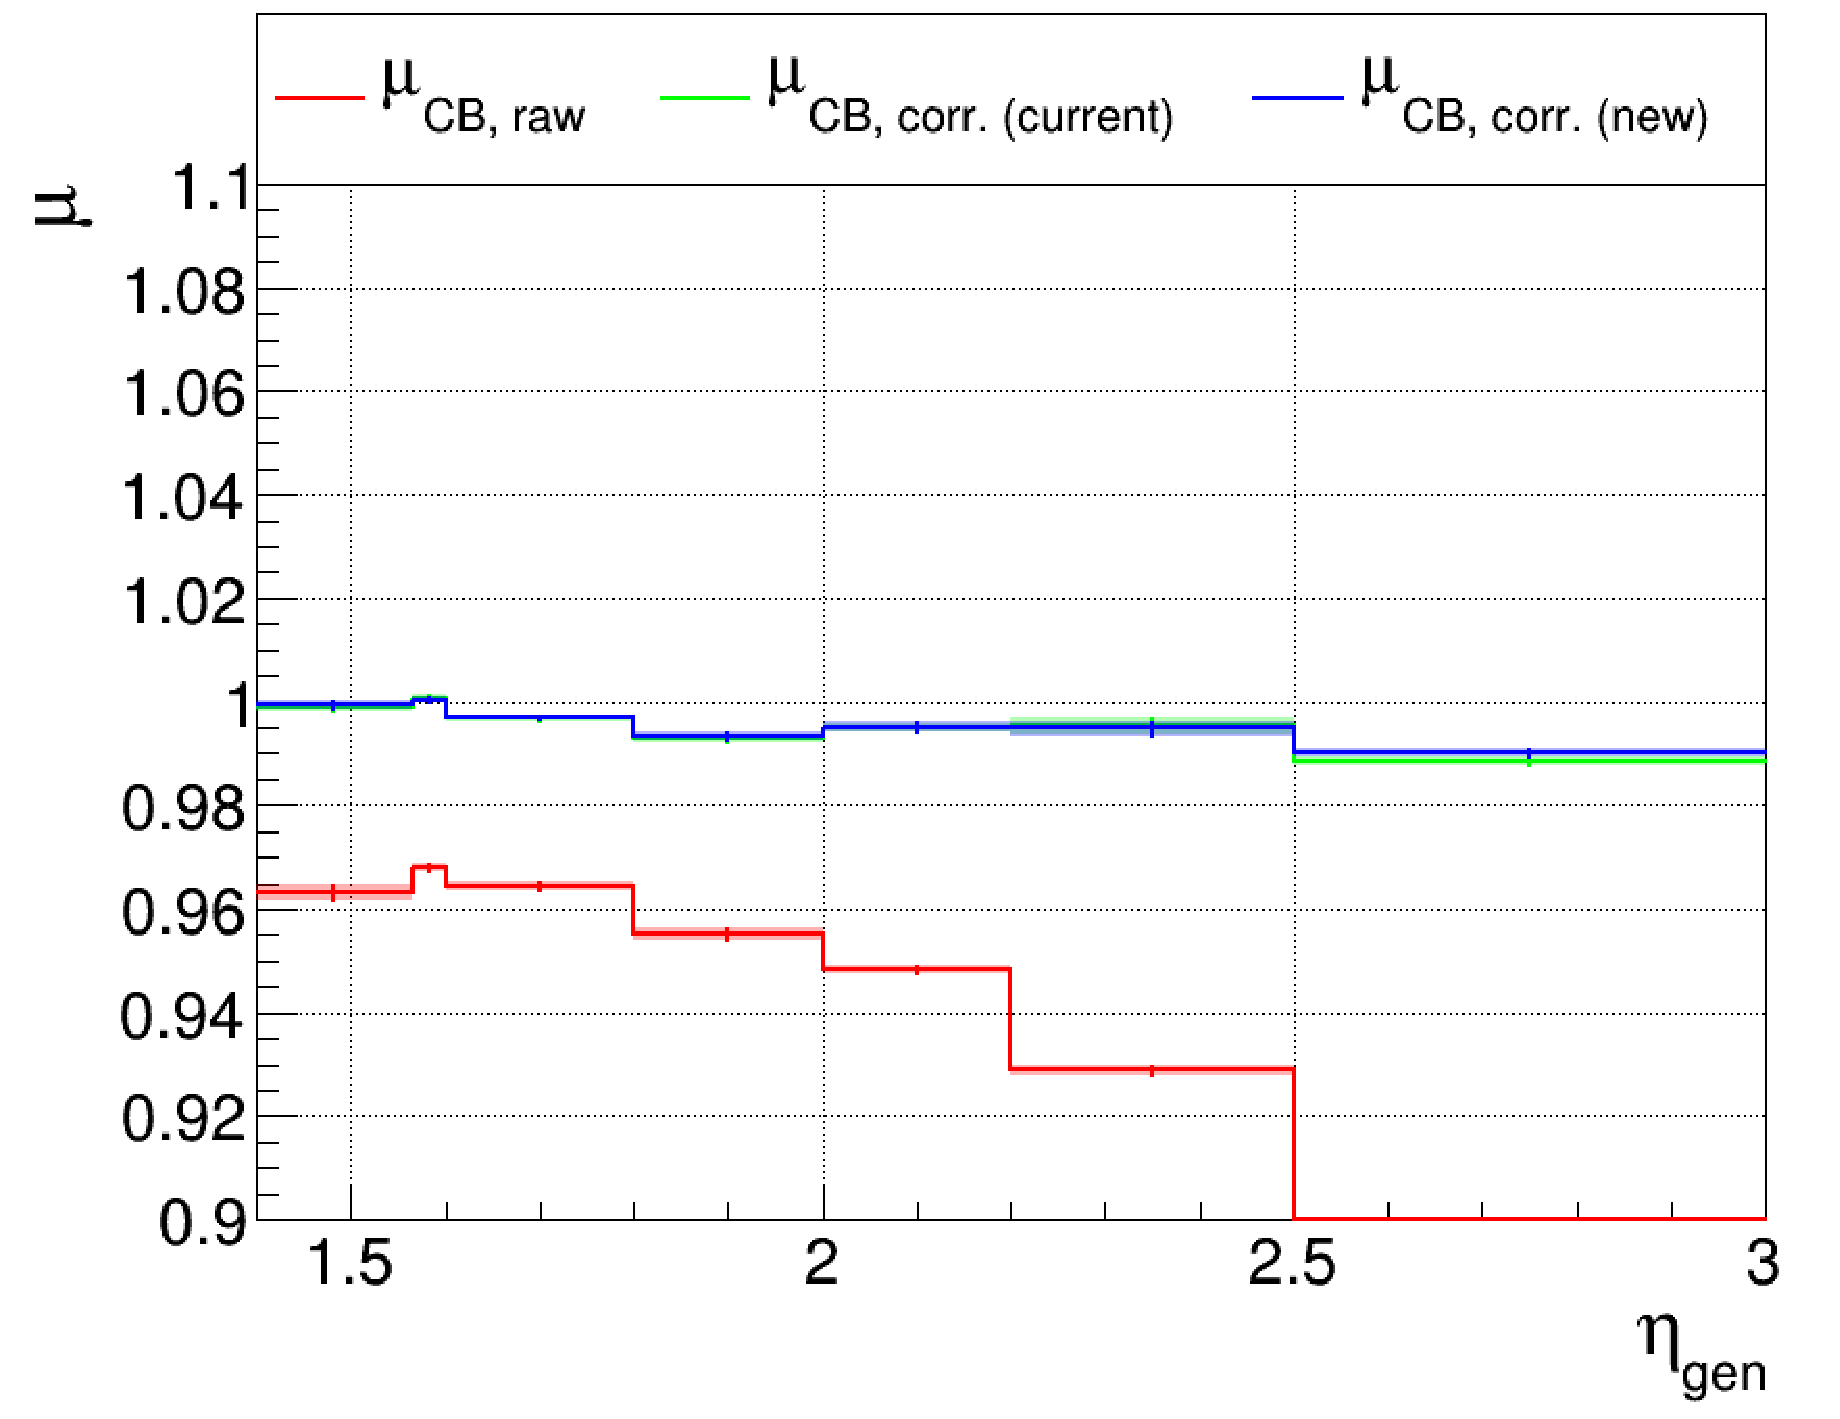
\includegraphics[width=0.495\textwidth]{./plots_pdf/ECAL_plots/plotsPU/EE/FULL/pdf/GENETA/EEFULL_GENETA_0020_0100_MuOverBins.pdf}
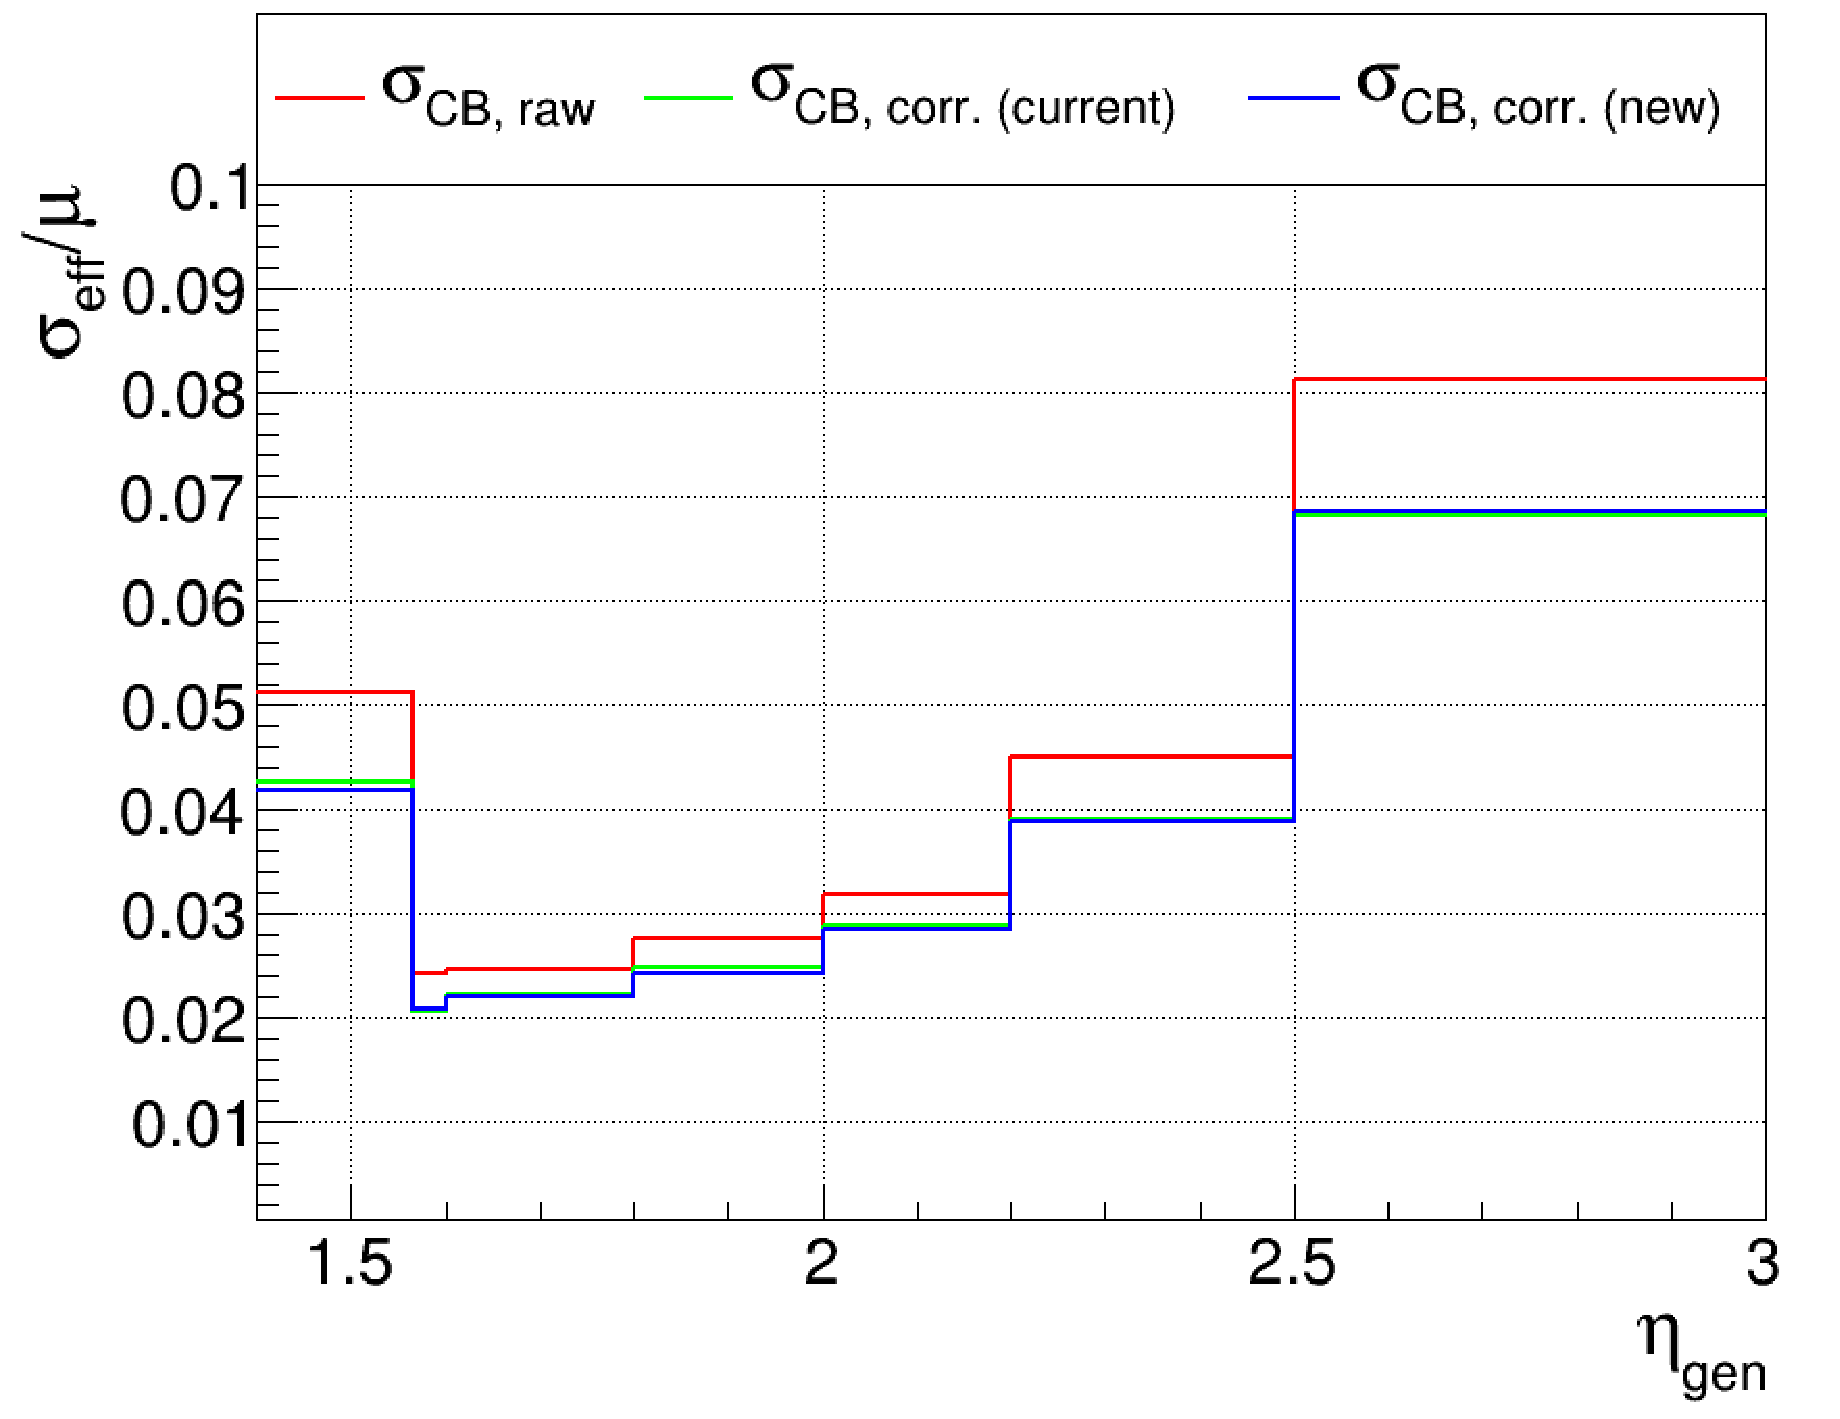
\includegraphics[width=0.495\textwidth]{./plots_pdf/ECAL_plots/plotsPU/EE/FULL/pdf/GENETA/EEFULL_GENETA_0020_0100_EffSigmaOverBins.pdf}
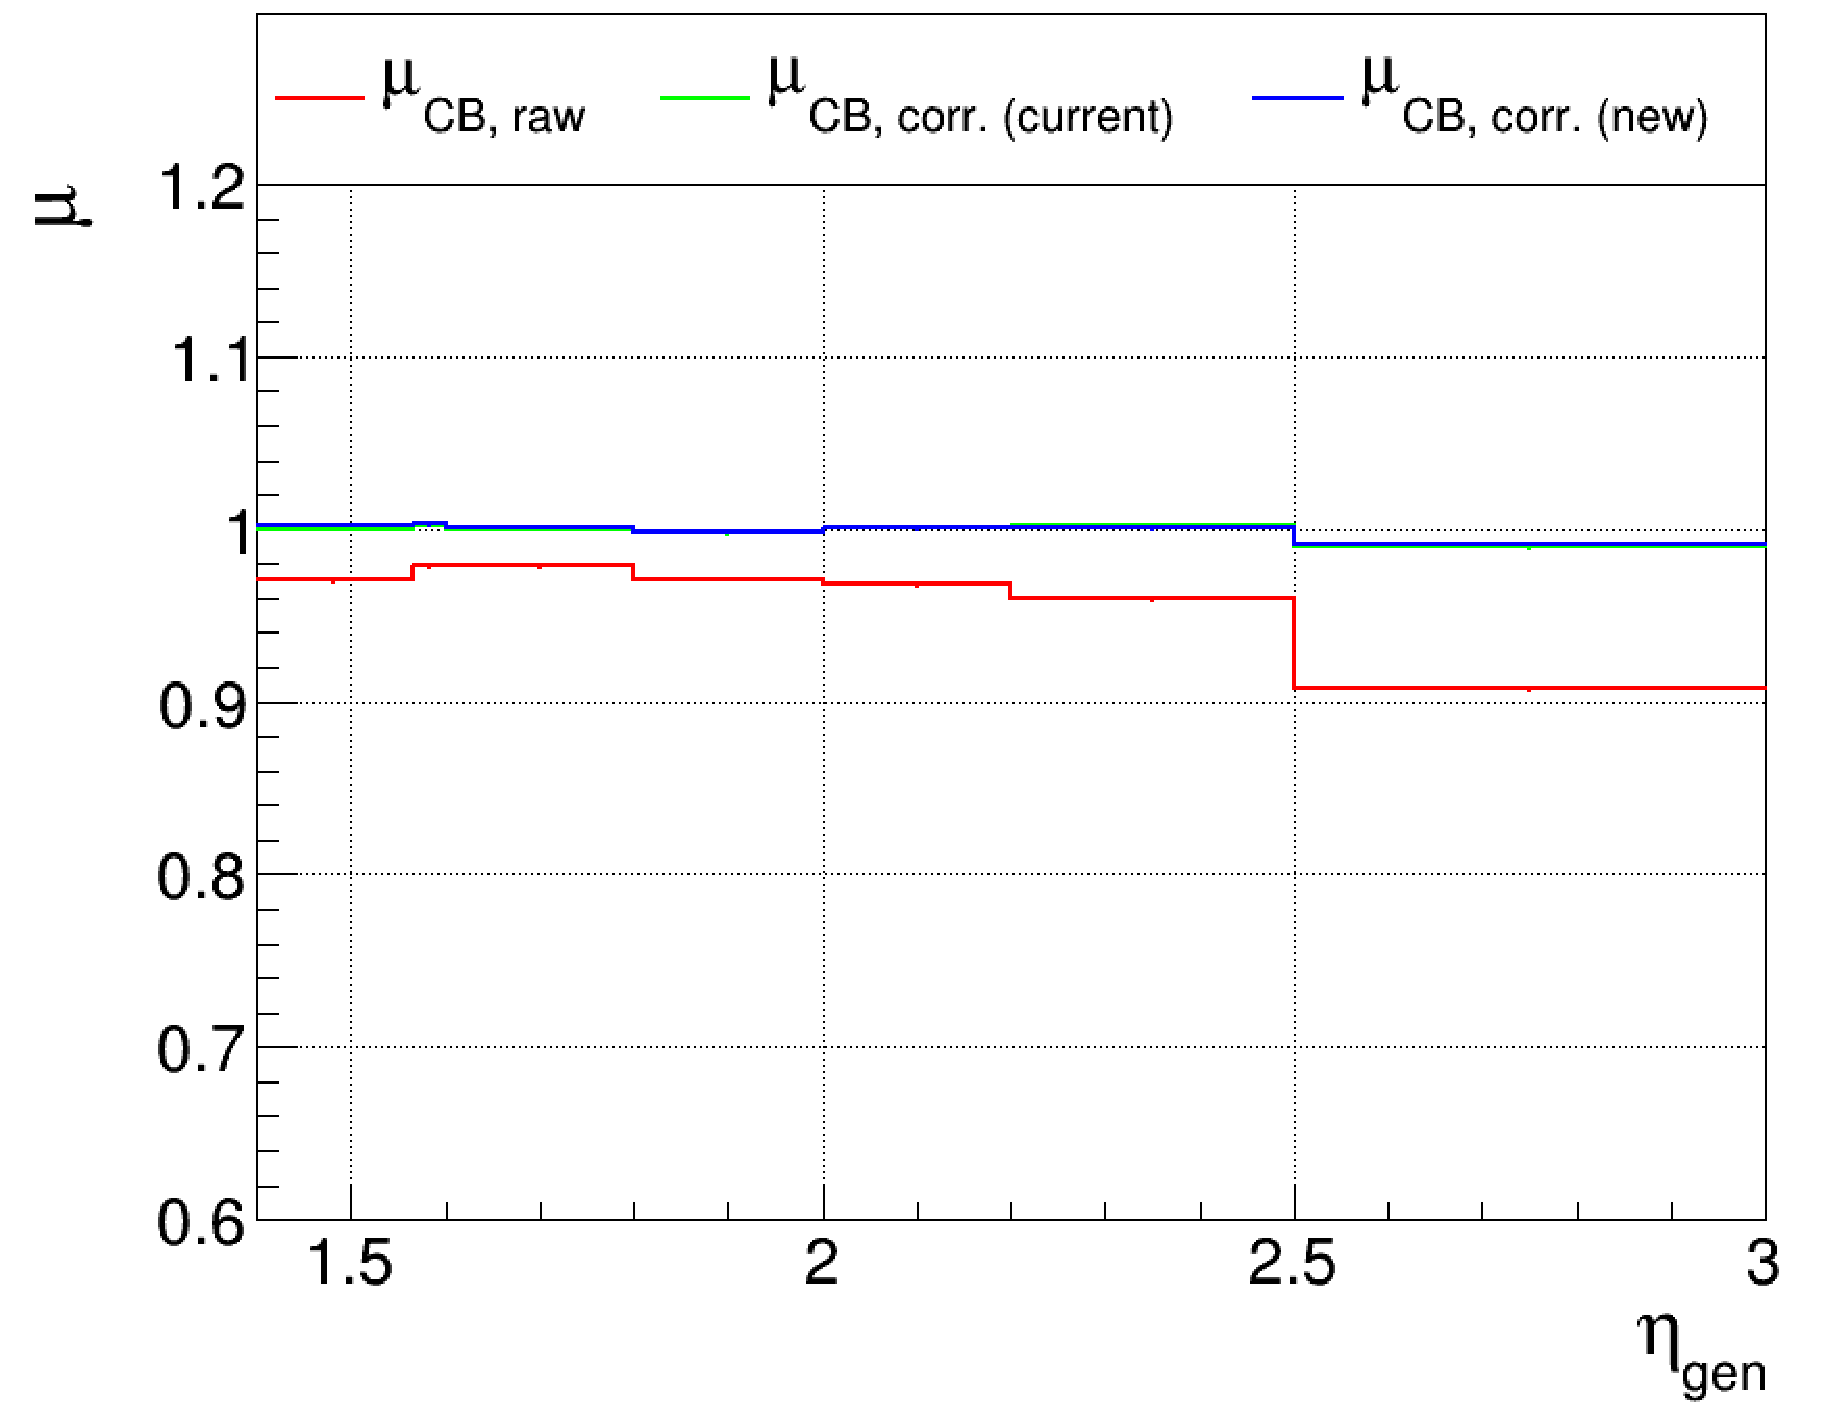
\includegraphics[width=0.495\textwidth]{./plots_pdf/ECAL_plots/plotsPU/EE/FULL/pdf/GENETA/EEFULL_GENETA_0100_0300_MuOverBins.pdf}
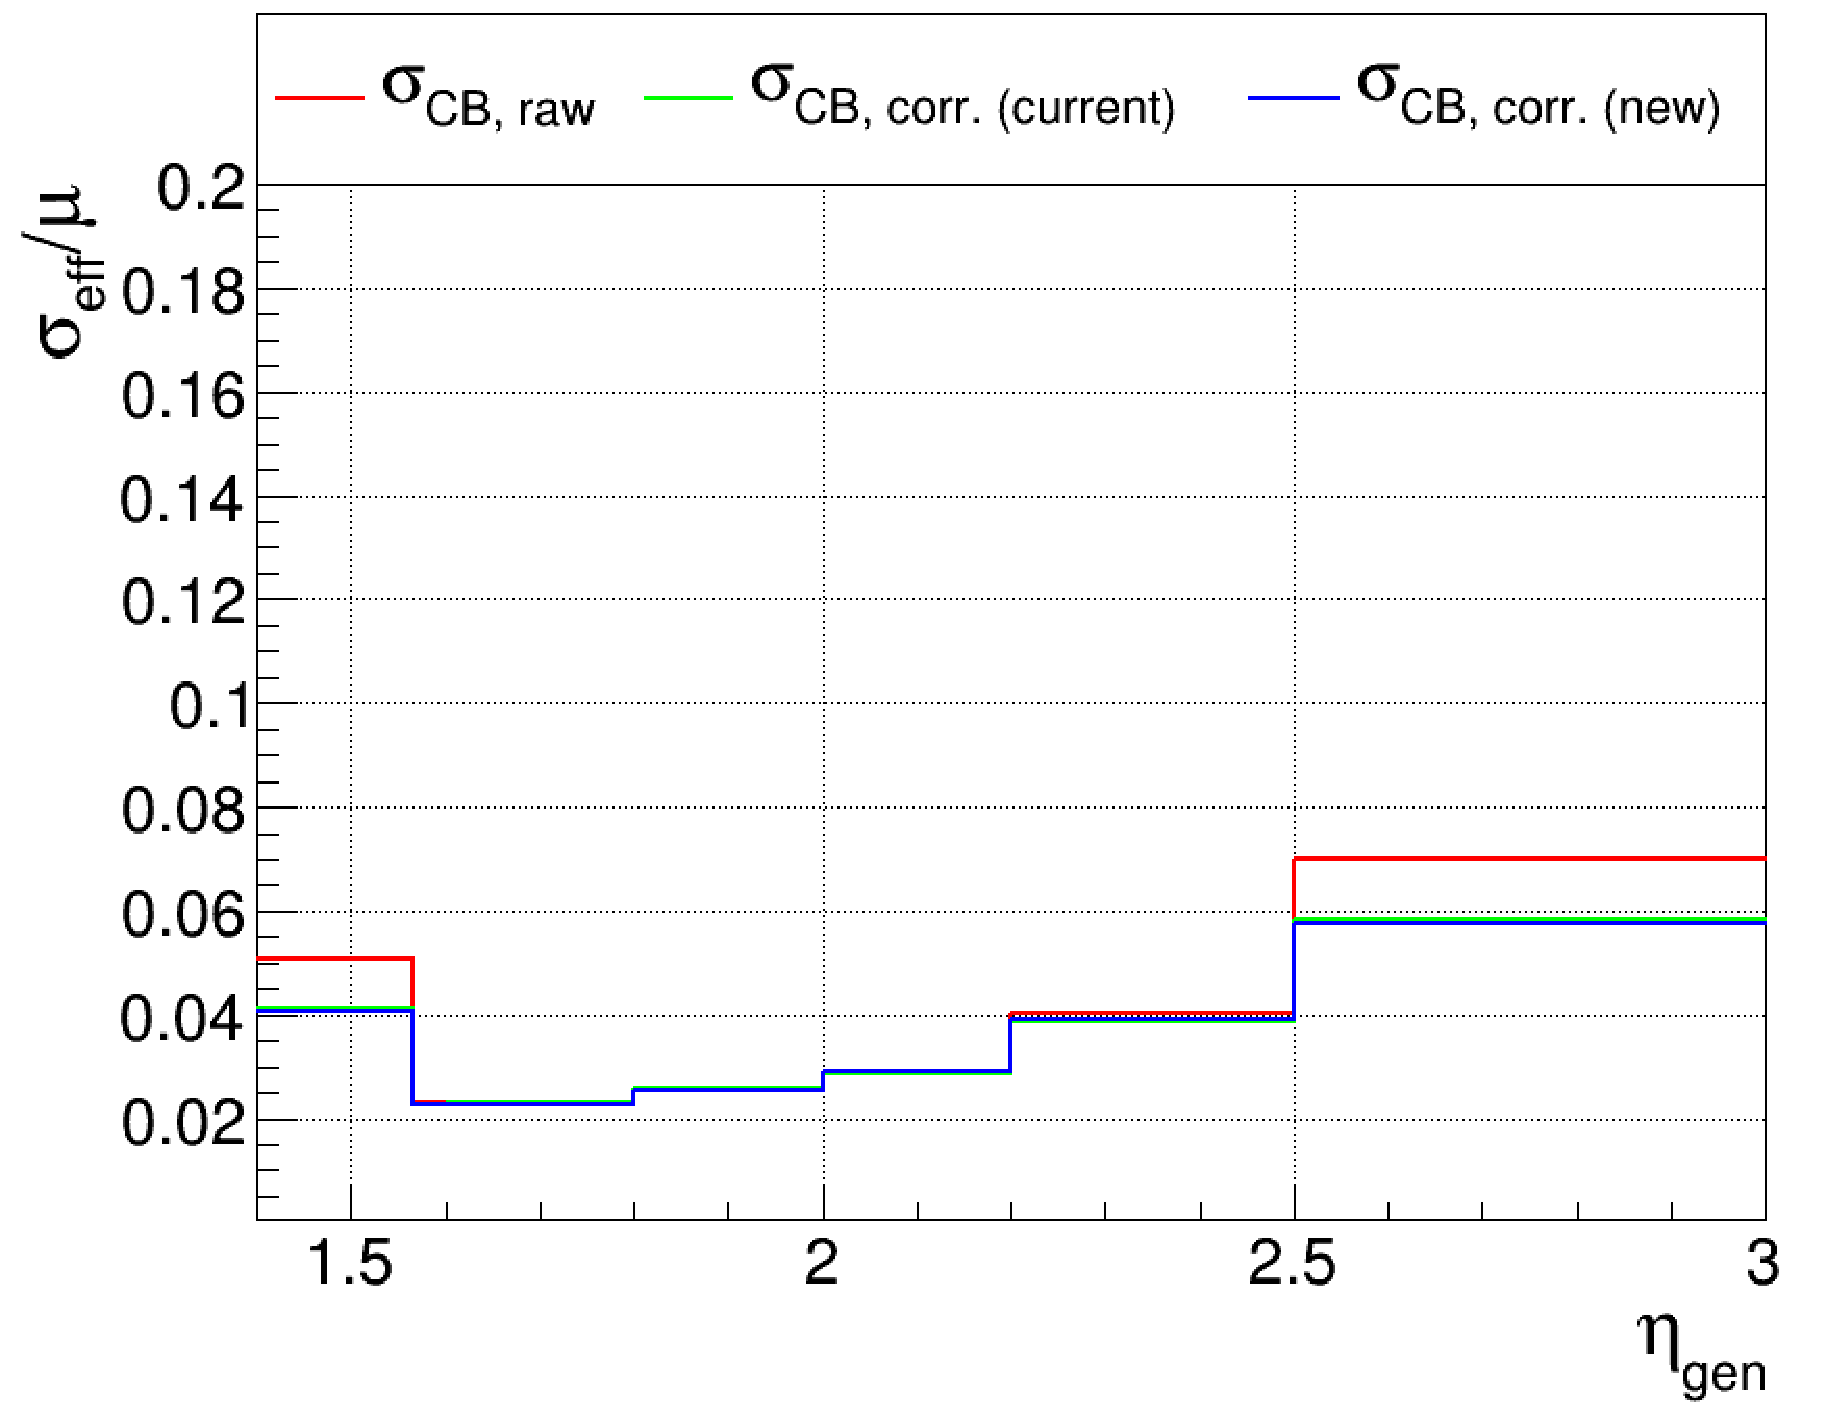
\includegraphics[width=0.495\textwidth]{./plots_pdf/ECAL_plots/plotsPU/EE/FULL/pdf/GENETA/EEFULL_GENETA_0100_0300_EffSigmaOverBins.pdf}


\caption [$\mu$ ($\sigma_\mathrm{eff}$) vs. $\eta$ of PF ECAL cluster - EE full readout PU scenario]{Mean response (resolution) defined by raw PF ECAL clusters (red), the calibration derived earlier in Run~3 based on 126X (green), and the new correction from the 2024 simulation sample based on 133X (blue). (top) low $\eta$, (middle) mid $\eta$, (bottom) high $\eta$ in EE region full readout PU scenario.}
\label{fig:PU_EEFULL_eta}
\end{figure}
